\documentclass[border=10pt]{standalone}
\usepackage{tikz}
\usetikzlibrary{calc}
\usepackage{xcolor}

\definecolor{lineA}{RGB}{0,100,180}    % blue
\definecolor{lineB}{RGB}{180,30,30}    % red
\definecolor{lineC}{RGB}{0,130,60}     % green

\begin{document}
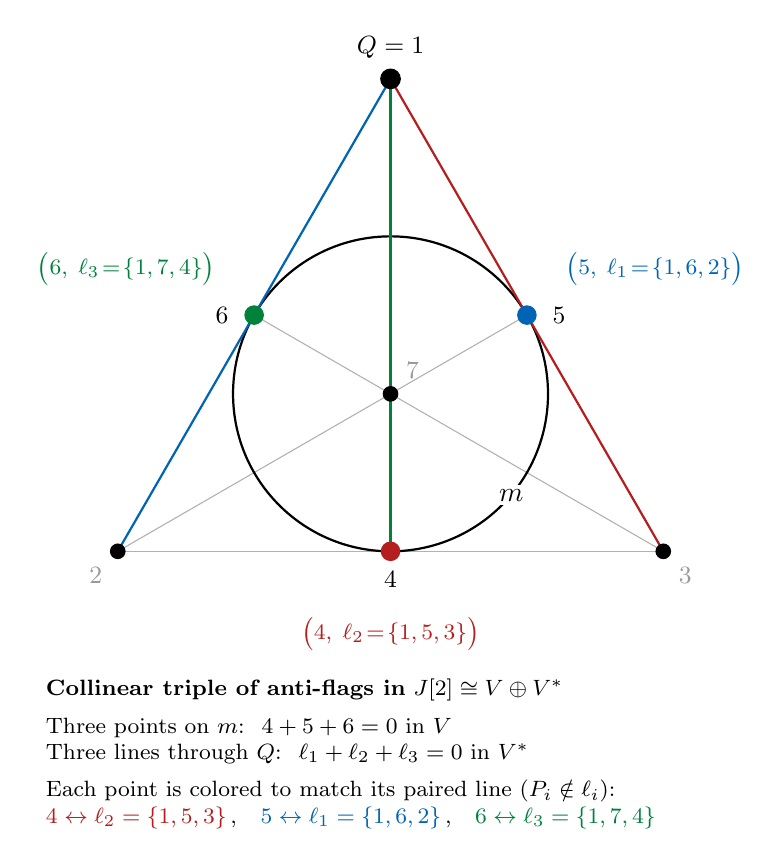
\begin{tikzpicture}[
    every node/.style={font=\small},
    point/.style={circle, fill, inner sep=2pt},
    antiflag point/.style={circle, fill=black, draw=black, inner sep=2.5pt},
    Q point/.style={circle, fill=black, draw=black, inner sep=2.5pt},
  ]

  % Coordinates: equilateral triangle, centroid at origin
  % Side length 4*sqrt(3), circumradius 4, nine-point radius 2
  \coordinate (1) at (0, 4);              % top vertex = Q
  \coordinate (2) at (-3.464, -2);        % bottom-left vertex
  \coordinate (3) at (3.464, -2);         % bottom-right vertex
  \coordinate (4) at (0, -2);             % midpoint of 2--3
  \coordinate (5) at (1.732, 1);          % midpoint of 1--3
  \coordinate (6) at (-1.732, 1);         % midpoint of 1--2
  \coordinate (7) at (0, 0);              % center

  % --- Other lines (not through Q), drawn first so they're behind ---
  % {2,4,3}: bottom side
  \draw[gray!60] (2) -- (3);
  % {2,7,5}: median from 2
  \draw[gray!60] (2) -- (5);
  % {3,7,6}: median from 3
  \draw[gray!60] (3) -- (6);

  % --- Line m = {4,5,6}: nine-point circle = incircle (equilateral) ---
  % Center = (0, 0), radius = 2; tangent to sides at midpoints
  \draw[thick, black] (0, 0) circle[radius=2];

  % --- Lines through Q = 1 (colored by anti-flag pairing) ---
  % ell_1 = {1,6,2}: left side -- paired with point 5
  \draw[thick, lineA] (1) -- (2);
  % ell_2 = {1,5,3}: right side -- paired with point 4
  \draw[thick, lineB] (1) -- (3);
  % ell_3 = {1,7,4}: vertical median -- paired with point 6
  \draw[thick, lineC] (1) -- (4);

  % --- Points ---
  % Q = point 1
  \node[Q point, label={above:$Q = 1$}] at (1) {};

  % Points on m: colored to match paired line
  \node[circle, fill=lineB, inner sep=2.5pt,
    label={below:$4$}] at (4) {};
  \node[circle, fill=lineA, inner sep=2.5pt,
    label={[anchor=west, xshift=2pt]right:$5$}] at (5) {};
  \node[circle, fill=lineC, inner sep=2.5pt,
    label={[anchor=east, xshift=-2pt]left:$6$}] at (6) {};

  % Other points
  \node[point, label={[gray!80]below left:$2$}] at (2) {};
  \node[point, label={[gray!80]below right:$3$}] at (3) {};
  \node[point, label={[gray!80]above right:$7$}] at (7) {};

  % --- Line m label, crossing the circle at lower-right ---
  \node[fill=white, inner sep=1.5pt, font=\normalsize] at (-40:2) {$m$};

  % --- Anti-flag annotations ---
  \node[lineB, anchor=north, font=\footnotesize] at (0, -2.7)
    {$\bigl(4,\; \ell_2\!=\!\{1,5,3\}\bigr)$};

  \node[lineA, anchor=west, font=\footnotesize] at (2.1, 1.6)
    {$\bigl(5,\; \ell_1\!=\!\{1,6,2\}\bigr)$};

  \node[lineC, anchor=east, font=\footnotesize] at (-2.1, 1.6)
    {$\bigl(6,\; \ell_3\!=\!\{1,7,4\}\bigr)$};

  % --- Legend ---
  \node[anchor=north west, align=left, font=\footnotesize] at (-4.5, -3.5) {
    \textbf{Collinear triple of anti-flags in} $J[2] \cong V \oplus V^*$\\[4pt]
    Three points on $m$: $\;4 + 5 + 6 = 0$ in $V$\\
    Three lines through $Q$: $\;\ell_1 + \ell_2 + \ell_3 = 0$ in $V^*$\\[4pt]
    Each point is colored to match its paired line ($P_i \notin \ell_i$):\\
    \textcolor{lineB}{$4 \leftrightarrow \ell_2 = \{1,5,3\}$}\,,\quad
    \textcolor{lineA}{$5 \leftrightarrow \ell_1 = \{1,6,2\}$}\,,\quad
    \textcolor{lineC}{$6 \leftrightarrow \ell_3 = \{1,7,4\}$}
  };

\end{tikzpicture}
\end{document}
